\documentclass[11pt]{article}

% --- packages ---
\usepackage[margin=1in]{geometry}
\usepackage{amsmath,amssymb}
\usepackage{algorithm}
\usepackage{algpseudocode}
\usepackage{booktabs}
\usepackage{hyperref}
\usepackage[capitalise,noabbrev]{cleveref}
\crefname{lstlisting}{Listing}{Listings}
\Crefname{lstlisting}{Listing}{Listings}
\usepackage{listings}
\usepackage{xcolor}
\usepackage{graphicx}
\usepackage{natbib}
\bibliographystyle{plainnat}

% --- listings style ---
\definecolor{jlstring}{rgb}{0.0,0.5,0.0}
\definecolor{jlcomment}{rgb}{0.5,0.5,0.5}
\definecolor{jlkeyword}{rgb}{0.0,0.0,0.7}
\lstset{
  language=Python, % closest built-in to Julia
  basicstyle=\small\ttfamily,
  keywordstyle=\color{jlkeyword}\bfseries,
  stringstyle=\color{jlstring},
  commentstyle=\color{jlcomment}\itshape,
  columns=fullflexible,
  keepspaces=true,
  breaklines=true,
  frame=single,
  numbers=left,
  numberstyle=\tiny\color{gray},
  morekeywords={function,end,using,for,if,elseif,else,return,while,push,true,false,export,module,include,struct},
  literate={::}{{\textcolor{gray}{::}}}2
           {=>}{{\textcolor{gray}{=>}}}2,
  escapeinside={(*@}{@*)},
}

% --- metadata ---
\title{ParetoEnsembles.jl: A Julia Package for Multiobjective Parameter Estimation Using Pareto Optimal Ensemble Techniques}
\author{
  Jeffrey D.\ Varner\thanks{Corresponding author: \texttt{jdv27@cornell.edu}}\\
  Robert Frederick Smith School of Chemical and Biomolecular Engineering\\
  Cornell University, Ithaca, NY 14853
}
\date{}

\begin{document}
\maketitle

% ============================================================
\begin{abstract}
Mathematical models of biological and engineering systems often have many adjustable parameters that must be estimated from multiple, potentially conflicting datasets.
Rather than reporting a single best-fit parameter vector, it is often more informative to generate an \emph{ensemble} of parameter sets that collectively map out the trade-offs among competing objectives.
ParetoEnsembles.jl is an open-source Julia package that generates such ensembles using Pareto Optimal Ensemble Techniques (POETs), a simulated-annealing-based algorithm that requires no gradient information and is defined entirely by four user-supplied callback functions.
This paper describes a substantially rewritten implementation that corrects the original dominance relation, reduces the per-iteration ranking cost through an incremental update scheme, and adds multi-chain parallel execution for improved front coverage.
We demonstrate the package on two standard benchmark problems, a cell-free gene expression model fitted to experimental data, and a blood coagulation cascade model with ten estimated rate constants and three objectives.
A head-to-head comparison with NSGA-II shows that ParetoEnsembles.jl produces denser fronts with comparable or superior hypervolume and inverted generational distance, and a sensitivity analysis confirms robustness to hyperparameter choices.
ParetoEnsembles.jl is available under the MIT license at \url{https://github.com/varnerlab/ParetoEnsembles.jl}.
\end{abstract}

\medskip
\noindent\textbf{Keywords:} multiobjective optimization, Pareto front, simulated annealing, ensemble methods, Julia, parameter estimation

% ============================================================
\section{Introduction}\label{sec:intro}
Mathematical models of biological and engineering systems typically contain many adjustable parameters that must be estimated from experimental data.
When multiple datasets measure different aspects of the same system --- for example, messenger RNA (mRNA) and protein concentrations in a gene expression circuit, or yield and selectivity in a reactor --- calibrating parameters to one dataset often degrades the fit to another, giving rise to a multiobjective optimization (MOO) problem~\citep{Miettinen1999,Deb2001,CoelloCoello2007}.
Compounding this difficulty, many models exhibit ``sloppy'' parameter sensitivities: broad, flat valleys in objective space where large regions of parameter space produce nearly equivalent fits~\citep{Gutenkunst2007}.
In such settings, reporting a single best-fit parameter vector obscures the practical uncertainty; instead, one needs an \emph{ensemble} of parameter sets that collectively map out the trade-offs among competing objectives.
The boundary of this ensemble in objective space is the Pareto front --- the set of solutions for which no objective can be improved without degrading at least one other --- and the full cloud of near-optimal solutions surrounding it characterizes the range of model behaviors consistent with the available data.

Several families of algorithms have been developed to approximate Pareto fronts.
Population-based evolutionary methods maintain a generation of candidate solutions that are selected, recombined, and mutated toward the front; prominent examples include the Non-dominated Sorting Genetic Algorithm II (NSGA-II)~\citep{Deb2002}, its many-objective successor NSGA-III~\citep{Deb2014}, and the Multiobjective Evolutionary Algorithm Based on Decomposition (MOEA/D), which decomposes the MOO problem into a set of scalar subproblems solved cooperatively~\citep{Zhang2007}.
An alternative trajectory-based strategy is multiobjective simulated annealing (SA), which extends the classical SA framework~\citep{Kirkpatrick1983} to multiple objectives by using Pareto dominance to guide acceptance decisions; early formulations include the Pareto SA method of~\citet{Czyzak1998} and the Archived Multiobjective Simulated Annealing (AMOSA) algorithm of~\citet{Bandyopadhyay2008}.
Pareto Optimal Ensemble Techniques (POETs), introduced by~\citet{Song2010} and later implemented in the Julia programming language as JuPOETs~\citep{Bassen2016}, belongs to this SA-based family; POETs ranks the current archive by counting how many other solutions dominate each candidate, then uses the rank as the energy in a Metropolis-type acceptance criterion.
Mature software implementations of these and related algorithms are available in several languages, including pymoo in Python~\citep{Blank2020} and Metaheuristics.jl in Julia~\citep{Mejia2022}, both of which focus primarily on population-based evolutionary strategies.

In this study, we present ParetoEnsembles.jl, a substantially rewritten Julia~\citep{Bezanson2017} implementation of the POETs algorithm.
The package takes a user-defined model and a set of objective functions --- each measuring how well a candidate parameter vector reproduces a particular dataset --- and returns a collection of parameter sets spanning the trade-off surface, along with their objective values and dominance ranks.
Several algorithmic corrections and performance improvements have been made relative to the original implementation: the dominance check has been corrected from weak to strict Pareto dominance, the per-iteration ranking cost has been reduced from $O(n^{2}m)$ to $O(nm)$ through an incremental update scheme (where $n$ is the archive size and $m$ is the number of objectives), and multi-chain parallel execution has been added to improve front coverage.
We describe the methods underlying ParetoEnsembles.jl (\cref{sec:methods}), present results on benchmark problems, two biological applications, and a comparison with NSGA-II (\cref{sec:results}), discuss the findings in the context of the broader multiobjective optimization landscape (\cref{sec:discussion}), and conclude with a summary and outlook (\cref{sec:conclusions}).

% ============================================================
\section{Methods}\label{sec:methods}

\subsection{Pareto dominance and ranking}\label{sec:dominance}
Consider an archive of $n$ solutions evaluated on $m$ objectives, where lower values are preferred.
Solution $\mathbf{x}_j$ \emph{strictly dominates} solution $\mathbf{x}_i$, written $\mathbf{x}_j \prec \mathbf{x}_i$, if and only if $f_k(\mathbf{x}_j) \leq f_k(\mathbf{x}_i)$ for all $k \in \{1,\ldots,m\}$ and there exists at least one objective $k$ for which $f_k(\mathbf{x}_j) < f_k(\mathbf{x}_i)$ (\cref{eq:dominance}).
The \emph{Pareto rank} of solution $\mathbf{x}_i$ is the number of archive members that strictly dominate it (\cref{eq:rank}), so that solutions with rank zero lie on the Pareto front and identical solutions --- which do not dominate each other under strict dominance --- share the same rank.
It is worth noting that the original POETs implementation~\citep{Song2010,Bassen2016} used \emph{weak} dominance, checking only that $f_k(\mathbf{x}_j) \leq f_k(\mathbf{x}_i)$ for all $k$ without requiring strict inequality in at least one objective; under weak dominance, identical solutions count as dominating each other, which inflates their ranks and causes excessive pruning of good solutions from the archive.
The current implementation enforces strict Pareto dominance, and the pairwise test iterates over objectives with an early-exit condition that terminates as soon as any objective of $j$ is found to be worse than $i$, avoiding unnecessary comparisons (\cref{alg:dominates}).
\begin{equation}\label{eq:dominance}
  f_k(\mathbf{x}_j) \leq f_k(\mathbf{x}_i) \quad \forall\, k \in \{1,\ldots,m\}
  \qquad\text{and}\qquad
  \exists\, k : f_k(\mathbf{x}_j) < f_k(\mathbf{x}_i).
\end{equation}
\begin{equation}\label{eq:rank}
  R(\mathbf{x}_i) = \bigl|\{\, j \neq i \mid \mathbf{x}_j \prec \mathbf{x}_i \,\}\bigr|.
\end{equation}

\subsection{Incremental ranking}\label{sec:incremental}
A central computational concern is the cost of ranking.
When a single candidate solution $\mathbf{x}_{\text{new}}$ is appended to an archive of $n-1$ existing solutions with known ranks $\mathbf{R}$, the na\"ive approach recomputes all $n(n-1)$ pairwise dominance checks at $O(n^2 m)$ cost.
Because only one solution changed, however, we can instead perform a single $O(nm)$ pass over the existing archive: for each existing solution $\mathbf{x}_i$, we test dominance in both directions, incrementing $R_i$ if the new solution dominates $\mathbf{x}_i$ and accumulating toward the new solution's rank if $\mathbf{x}_i$ dominates it.
This incremental procedure (\cref{alg:rankinsert}) reduces the per-iteration cost from $O(n^2 m)$ to $O(nm)$, with a full $O(n'^2 m)$ re-rank performed only after archive pruning when $n'$ is small.

\subsection{Pareto simulated annealing}\label{sec:annealing}
The complete Pareto simulated annealing procedure combines the dominance check and incremental ranking into a single outer-inner loop structure (\cref{alg:main}).
The algorithm is seeded with an initial parameter vector $\mathbf{x}_0$, an initial temperature $T = 1$, and an archive containing the single evaluated solution $(\mathbf{x}_0, \mathbf{f}(\mathbf{x}_0))$.
At each temperature level, $N_{\text{iter}}$ candidate solutions are generated by perturbing the current best parameter vector through a user-supplied neighbor function, and the rank array is updated incrementally via \textsc{RankInsert} at $O(nm)$ cost per candidate.
The acceptance probability, computed from the rank array and the current temperature, determines whether the candidate is retained; upon acceptance, solutions whose rank meets or exceeds the cutoff $R_{\text{cutoff}}$ are pruned and a full re-rank is performed on the smaller remaining set, with a hard size cap $n_{\max}$ enforced if the archive still exceeds the limit.
Upon rejection, the candidate is immediately removed and the rank array is restored from a saved snapshot, a strategy we refer to as \emph{pop-on-reject}; in the original implementation, rejected candidates remained in the archive, causing unbounded growth of $n$ between accepted moves and progressively more expensive ranking operations, and the pop-on-reject strategy eliminates this problem entirely.

\subsection{Parallel execution}\label{sec:parallel}
Two opportunities for parallelism arise from the structure of the algorithm.
First, the outer loop of both the full ranking and the incremental \textsc{RankInsert} procedure iterates independently over archive solutions, so setting \texttt{parallel\_evaluation=true} dispatches to threaded variants that distribute these independent iterations across available threads using Julia's \texttt{Threads.@threads} construct, with an atomic accumulator used for $R_{\text{new}}$ in the incremental case since multiple threads contribute to it.
Second, and more significantly, because simulated annealing is inherently sequential within a single chain, the most effective parallelization strategy is to run $C$ independent chains from different starting points and merge the resulting archives (\cref{alg:multichain}); each chain receives its own deterministic random number generator seeded from a base seed and the chain index, ensuring reproducibility, and after all chains complete, the archives are concatenated and a final full ranking is performed on the merged set.

\subsection{Software design}\label{sec:software}
ParetoEnsembles.jl is a pure Julia package with no dependencies beyond the standard library module \texttt{Random}, and its public API consists of five functions (\cref{tab:api}).
The primary entry point, \texttt{estimate\_ensemble}, runs a single Pareto SA chain and returns the retained objective values, parameter vectors, and Pareto ranks; its parallel counterpart, \texttt{estimate\_ensemble\_parallel}, runs $C$ independent chains concurrently, merges their archives, and re-ranks the combined set.
A standalone \texttt{rank\_function} computes Pareto ranks for an arbitrary $m \times n$ objective matrix and can be used independently of the optimization loop, while \texttt{hypervolume} computes the hypervolume indicator for a 2D front using a sweep-line algorithm in $O(n \log n)$ time and \texttt{pareto\_front} extracts the rank-zero subset from the archive for downstream analysis.

The algorithm is entirely defined by four user-supplied callback functions (\cref{tab:callbacks}): an objective function that maps a parameter vector $\mathbf{x} \in \mathbb{R}^d$ to an $m \times 1$ array of objective values, a neighbor function that perturbs a given parameter vector to generate a candidate, an acceptance probability function that returns a scalar probability from the rank array and temperature, and a cooling function that maps the current temperature to a reduced value.
Beyond these four callbacks, the behavior of \texttt{estimate\_ensemble} is controlled by keyword arguments including the pruning threshold \texttt{rank\_cutoff} (default~5), the number of candidates per temperature level \texttt{maximum\_number\_of\_iterations} (default~20), the stopping temperature \texttt{temperature\_min} (default $10^{-4}$), and the hard archive size cap \texttt{maximum\_archive\_size} (default~1000).
When \texttt{trace=true}, the algorithm records convergence diagnostics --- temperature, archive size, and hypervolume --- at each cooling step, returning a fourth element in the output tuple that allows users to monitor convergence and assess whether the annealing schedule was sufficient.
Representative Julia code demonstrating both the single-chain and multi-chain interfaces is provided in the Supplementary Material (\cref{lst:binhkorn,lst:parallel}).

% ============================================================
\section{Results}\label{sec:results}

\subsection{Standard benchmarks}\label{sec:benchmarks}
We first demonstrate ParetoEnsembles.jl on two standard multiobjective benchmarks: the constrained Binh--Korn problem~\citep{Binh1997} (\cref{eq:bk_obj}) and the unconstrained Fonseca--Fleming problem~\citep{Fonseca1995} with $d = 3$ decision variables (\cref{eq:ff}).
Constraints in the Binh--Korn problem are enforced via quadratic penalty terms added to the objective values, and bound constraints are handled by clamping in the neighbor function.
We ran both benchmarks using ten parallel chains with $N_{\text{iter}} = 60$, $R_{\text{cutoff}} = 12$, and $\alpha = 0.95$, and the resulting Pareto fronts in objective space recover the characteristic trade-off curves for both problems, with a visible cloud of near-optimal solutions surrounding the non-dominated front (\cref{fig:benchmarks}a,b).
The computed front for the Fonseca--Fleming case lies directly on the theoretical curve, confirming that the algorithm converges to the correct solution set, and in parameter space the Binh--Korn Pareto-optimal decision vectors trace a curved manifold from the origin toward $(5, 3)$ while the Fonseca--Fleming solutions cluster along the diagonal $x_1 \approx x_2$ as expected from the symmetric structure of the objectives (\cref{fig:benchmarks}c,d).
Comparing a single chain against ten parallel chains on the Binh--Korn problem illustrates the benefit of multi-chain execution (\cref{fig:parallel}): the single chain recovers the trade-off curve but, because every retained solution is non-dominated within that chain's archive, the rank array contains only rank-zero entries, whereas the merged multi-chain run produces a denser front with broader coverage of the feasible region.
\begin{align}
  \min_{\mathbf{x}} \quad & f_1 = 4x_1^2 + 4x_2^2, \qquad f_2 = (x_1 - 5)^2 + (x_2 - 5)^2 \label{eq:bk_obj} \\
  \text{s.t.} \quad & (x_1 - 5)^2 + x_2^2 \leq 25, \qquad (x_1 - 8)^2 + (x_2 - 3)^2 \geq 7.7 \notag \\
  & 0 \leq x_1 \leq 5, \quad 0 \leq x_2 \leq 3. \notag
\end{align}
\begin{equation}\label{eq:ff}
  f_1(\mathbf{x}) = 1 - \exp\!\Biggl(-\sum_{i=1}^{d}\Bigl(x_i - \tfrac{1}{\sqrt{d}}\Bigr)^{\!2}\Biggr), \qquad
  f_2(\mathbf{x}) = 1 - \exp\!\Biggl(-\sum_{i=1}^{d}\Bigl(x_i + \tfrac{1}{\sqrt{d}}\Bigr)^{\!2}\Biggr).
\end{equation}

\subsection{Cell-free gene expression}\label{sec:cellfree}
As a first biological application, we considered the estimation of kinetic parameters for a cell-free gene expression circuit describing the production of deGFP protein driven by the endogenous sigma factor $\sigma_{70}$ via the P70 promoter, following the effective biophysical framework of~\citet{Adhikari2020}.
The system is governed by two ordinary differential equations for mRNA ($m$) and protein ($p$), where $\dot{m} = \alpha\, u(\sigma_{70}) - \delta_m\, m$ and $\dot{p} = \kappa\, m\, w(t) - \delta_p\, p$, with $u(\sigma_{70}) = \sigma_{70}^{n}/(K^n + \sigma_{70}^n)$ representing a Hill-type promoter activity function and $w(t) = \exp(-\ln 2 \cdot t / \tau_{1/2})$ capturing the experimentally observed decay of translational capacity over the course of the cell-free reaction.
Five parameters were treated as unknown --- the maximum transcription rate $\alpha$, the effective translation rate constant $\kappa$, the mRNA degradation rate $\delta_m$, the promoter dissociation constant $K$, and the translation capacity half-life $\tau_{1/2}$ --- while the remaining parameters ($\sigma_{70} = 35$~nM, $n = 1.5$, $\delta_p = 0.005$~h$^{-1}$) were fixed at values taken from the literature.

We fitted the model to experimental data from~\citet{Adhikari2020}, consisting of mRNA and deGFP protein concentrations measured at five time points (0, 2, 4, 8, and 16~h) in triplicate, with reported means and standard deviations.
Two objectives were defined as standard-deviation-weighted sums of squared errors: $\varepsilon_{\text{mRNA}} = \sum_i [(m_i^{\text{sim}} - m_i^{\text{obs}}) / \sigma_i^m]^2$ and $\varepsilon_{\text{protein}} = \sum_i [(p_i^{\text{sim}} - p_i^{\text{obs}}) / \sigma_i^p]^2$, and we ran ten parallel chains with $R_{\text{cutoff}} = 8$ and $N_{\text{iter}} = 50$, starting from random initial parameter vectors drawn uniformly within the bounds.
The resulting ensemble captured the dynamics of both mRNA and protein expression (\cref{fig:cellfree}a,b): the 95\% confidence interval of the ensemble simulations bracketed the experimental data at all time points, and the ensemble mean tracked the observed trajectories.
The Pareto front revealed a clear trade-off between fitting the mRNA and protein time courses (\cref{fig:cellfree}c), with parameter sets that minimized $\varepsilon_{\text{mRNA}}$ tending to have slightly larger $\varepsilon_{\text{protein}}$ and vice versa --- a trade-off that arises naturally because the mRNA degradation rate and translation capacity half-life have opposing effects on the two species, so that the ensemble provides a family of plausible parameter sets rather than a single point estimate, enabling downstream uncertainty quantification of model predictions.

\subsection{Blood coagulation cascade}\label{sec:coag}
To demonstrate the package on a larger-scale system, we considered the Hockin--Mann model of tissue-factor-initiated blood coagulation~\citep{HockinMann2002}, a mechanistic ODE model describing 34 chemical species interacting through 27 reactions governed by 42 rate constants that captures the initiation, amplification, and inhibition phases of thrombin generation.
All rate constants are available in the literature and were used as ground truth, and we selected ten key catalytic and inhibition rate constants for estimation spanning the extrinsic factor Xase ($k_{\text{cat}}$), intrinsic factor Xase ($k_{\text{cat}}$), prothrombinase ($k_{\text{cat}}$), and antithrombin~III inhibition pathways.
Because these rate constants span six orders of magnitude (from $\sim$1 to $\sim 10^7$), we worked in log-space with bounds of $\pm 1.5$ orders of magnitude around the true values, and generated noisy ``experimental'' data by simulating the model with the true rate constants at two tissue factor (TF) concentrations (5~pM and 25~pM) and adding 10\% multiplicative Gaussian noise to the total thrombin trajectory.
Three objectives were defined: the normalized sum-of-squared error of the thrombin trajectory at 5~pM TF, the normalized SSE at 25~pM TF, and a regularization term measuring the mean squared log-distance of estimated rate constants from their literature values.

We ran eight parallel chains with $R_{\text{cutoff}} = 10$, $N_{\text{iter}} = 40$, and $\alpha = 0.92$, and the resulting ensemble of 140 parameter sets (rank $\leq 1$) produced thrombin trajectories that closely matched the noisy data at both TF concentrations (\cref{fig:coag}a,b).
Parameter recovery was strong: median estimates for 8 of 10 rate constants fell within 10\% of the true values, with the prothrombinase $k_{\text{cat}}$ and antithrombin inhibition rates recovered to within 1--5\% (\cref{fig:coag}c), while the hardest parameter to recover was the Factor~VIIIa activation rate ($k_{\text{IIa} \to \text{VIIIa}}$, 45\% error), reflecting its weaker influence on the thrombin trajectory relative to the dominant prothrombinase pathway.
The three-dimensional Pareto front (\cref{fig:coag}d) revealed the expected trade-off between fitting the two TF conditions and staying close to the literature values, demonstrating that ParetoEnsembles.jl scales effectively to systems with tens of species, ten or more estimated parameters, and three competing objectives.

\subsection{Ensemble-based prediction and identifiability analysis}\label{sec:ensemble_insights}
A key advantage of generating parameter ensembles rather than single point estimates is the ability to propagate uncertainty forward through the model to obtain calibrated prediction intervals.
To demonstrate this, we used the coagulation ensemble --- which was trained only on thrombin trajectories at 5~pM and 25~pM TF --- to predict the thrombin time course at a held-out tissue factor concentration of 1~pM that was never used during optimization.
The ensemble mean predicted a peak thrombin concentration of 497~nM, within 2\% of the true value of 508~nM, and the 95\% prediction interval from the ensemble bracketed the true trajectory along its entire time course (\cref{fig:insights}a).
By contrast, the single best-fit parameter vector (lowest combined training error) produced a comparable point prediction but provided no uncertainty information whatsoever, illustrating why ensemble methods are essential when model predictions will inform downstream decisions.

The ensemble also reveals the identifiability structure of the estimated parameters through their pairwise correlations (\cref{fig:insights}b).
The strongest correlation was between the extrinsic factor Xase $k_{\text{cat}}$ and the prothrombinase $k_{\text{cat}}$ ($r = -0.80$), indicating that these two catalytic rates compensate each other: if the initiation-phase enzyme is faster, the amplification-phase enzyme must be correspondingly slower to produce the same thrombin trajectory.
Other mechanistically interpretable correlations included the direct Xa-mediated thrombin generation rate versus Factor~Va activation ($r = -0.51$), reflecting the competition between direct and prothrombinase-mediated pathways, and the Factor~IXa activation rate versus the prothrombinase $k_{\text{cat}}$ ($r = -0.55$), reflecting the coupling between the intrinsic tenase and prothrombinase complexes in the amplification loop.
These compensatory relationships, which are invisible to single-point estimation methods, provide mechanistic insight into which parameter combinations the data can and cannot constrain.

Finally, we used the ensemble to simulate a clinically relevant perturbation: Factor~VIII deficiency (hemophilia~A) at varying severity levels.
By reducing the initial Factor~VIII concentration to 30\% (mild hemophilia) and 5\% (severe hemophilia) of the nominal plasma level while keeping all estimated rate constants at their ensemble values, we obtained patient-specific predictions of thrombin generation that captured both the expected dose-dependent reduction in peak thrombin and the associated uncertainty (\cref{fig:insights}c).
Peak thrombin decreased from $633 \pm 9$~nM in normal plasma to $517 \pm 8$~nM for mild hemophilia and $376 \pm 10$~nM for severe hemophilia, with the ensemble prediction intervals providing a quantitative measure of the confidence one should place in these predictions given the uncertainty in the underlying rate constants.
Importantly, the true trajectories (computed from the known ground-truth parameters) fell within the ensemble prediction bands for all three conditions, confirming that the uncertainty estimates are well calibrated even for conditions that were not part of the original training data.

\subsection{Comparison with NSGA-II}\label{sec:nsga}
To position ParetoEnsembles.jl relative to population-based evolutionary methods, we compared it against NSGA-II~\citep{Deb2002} as implemented in Metaheuristics.jl~\citep{Mejia2022} on both benchmark problems, matching the function evaluation budget at approximately 110{,}000 evaluations per solver (ParetoEnsembles: 10 chains, $N_{\text{iter}} = 60$, $\alpha = 0.95$; NSGA-II: population 200, 550 generations).
Five independent replicates were run for each solver, and the median hypervolume indicator (HV) and inverted generational distance (IGD) are reported in \cref{tab:comparison}, with IGD computed against the analytical Pareto front for the Fonseca--Fleming problem and against a densely sampled reference front from a high-budget run for Binh--Korn.
ParetoEnsembles.jl achieved comparable or slightly higher hypervolume than NSGA-II on both problems and substantially lower IGD --- 5$\times$ lower on Binh--Korn and 7$\times$ lower on Fonseca--Fleming --- indicating a closer approximation to the true Pareto front (\cref{fig:comparison}), while also producing much denser fronts with 2{,}000--6{,}000 non-dominated solutions compared with 200 for NSGA-II, reflecting its design as an ensemble generator that characterizes the full cloud of near-optimal solutions rather than merely approximating the front boundary.
NSGA-II was 50--150$\times$ faster in wall time, consistent with its population-parallel evaluation strategy, but this speed advantage comes at the cost of a sparser representation of the trade-off surface that may be insufficient for downstream uncertainty analysis.

\subsection{Hyperparameter sensitivity}\label{sec:sensitivity}
We assessed the sensitivity of ParetoEnsembles.jl to three key hyperparameters --- rank cutoff $R_{\text{cutoff}}$, cooling rate $\alpha$, and iterations per temperature $N_{\text{iter}}$ --- by sweeping each while holding the others at default values ($R_{\text{cutoff}} = 8$, $\alpha = 0.90$, $N_{\text{iter}} = 40$) on the Binh--Korn benchmark with five chains and five replicates per configuration (\cref{fig:sensitivity}).
The hypervolume indicator was robust across all tested ranges: rank cutoff values from 2 to 12 produced nearly identical results, with a modest decline at $R_{\text{cutoff}} = 20$ where the archive retains many low-quality solutions; faster cooling ($\alpha = 0.80$) performed comparably to slower cooling ($\alpha = 0.95$), with the latter showing slightly more variability; and even 10 iterations per temperature level produced competitive fronts, though 20 or more reduced inter-replicate variance.
These results suggest that the default hyperparameters provide a reasonable starting point for most problems, and that users need not invest significant effort in tuning --- a practical advantage for the systems biology applications where ParetoEnsembles.jl is primarily intended to be used.

\subsection{Parallel scaling}\label{sec:scaling}
To quantify the benefit of multi-chain parallelism, we measured wall clock time for the cell-free ensemble estimation (ten chains, $N_{\text{iter}} = 50$) as a function of the number of Julia threads (\cref{tab:scaling}).
Each configuration was run five times and the median time is reported; the speedup is approximately linear up to four threads ($3.1\times$) and reaches $4.1\times$ at eight threads, with diminishing returns due to load imbalance when ten chains are distributed across eight threads and the serial cost of the final archive merge and re-ranking step.

% ============================================================
\section{Discussion}\label{sec:discussion}
ParetoEnsembles.jl provides a lightweight Julia implementation of Pareto Optimal Ensemble Techniques for multiobjective optimization that addresses several limitations of the original POETs algorithm~\citep{Song2010,Bassen2016}.
The current version corrects the dominance relation from weak to strict, reduces the per-iteration ranking cost from $O(n^2 m)$ to $O(nm)$ through incremental updating, bounds archive growth through the pop-on-reject strategy and a hard size cap, adds both threaded ranking and multi-chain parallel execution, and provides built-in hypervolume computation and convergence diagnostics.
The callback-based design decouples the optimization algorithm from the problem definition, allowing users to apply ParetoEnsembles.jl to any domain where objective functions can be evaluated pointwise, and the head-to-head comparison with NSGA-II demonstrates that this SA-based approach achieves comparable hypervolume and substantially better IGD while producing fronts that are 10--30$\times$ denser than those returned by a leading evolutionary method at matched evaluation budgets.
While NSGA-II is considerably faster in wall time --- reflecting the inherently sequential nature of SA chains versus the population-parallel evaluation of evolutionary methods --- ParetoEnsembles.jl targets problems where the primary goal is to characterize the \emph{cloud} of near-optimal parameter sets, not just the front itself, and where the simplicity of the interface lowers the barrier to generating parameter ensembles as part of a modeling workflow.

The biological applications presented here illustrate both the strengths and the current scope of the package.
The cell-free gene expression example demonstrates that even a small model with five parameters and two objectives can reveal meaningful trade-offs when fitted to real experimental data, and the coagulation cascade example shows that the approach scales to systems with 34 species, ten estimated parameters spanning six orders of magnitude, and three competing objectives, recovering most rate constants to within 10\% of their true values.
Crucially, the downstream analyses of the coagulation ensemble --- held-out prediction, parameter identifiability, and patient-specific simulation --- demonstrate that the value of an ensemble extends far beyond the optimization itself.
The ensemble predicted thrombin generation at a held-out TF concentration to within 2\% of the true peak, with well-calibrated 95\% prediction intervals that no single point estimate can provide; the pairwise parameter correlations revealed mechanistically interpretable compensatory relationships between catalytic rate constants in the initiation and amplification phases of coagulation; and the hemophilia~A simulations showed that the ensemble can propagate parametric uncertainty through clinically relevant perturbations, yielding prediction intervals that widen appropriately as the system is driven further from the training conditions.
These capabilities illustrate why ensemble methods are essential in applications where model predictions inform consequential decisions, and they provide a template for how ParetoEnsembles.jl can be used in practice.
The hyperparameter sensitivity analysis further shows that the algorithm is robust to the choice of rank cutoff, cooling rate, and iterations per temperature, so that users can adopt the default settings without extensive tuning, and the convergence trace feature provides a built-in diagnostic for monitoring whether the annealing schedule was sufficient.

Several features are deliberately omitted from the current scope.
The package does not implement gradient-based refinement, surrogate modeling, or adaptive cooling schedules, nor does it provide built-in visualization or benchmark problem libraries.
Integration with Julia's automatic differentiation ecosystem, for example through ForwardDiff.jl or Enzyme.jl, could enable hybrid gradient-free/gradient-based strategies for problems where gradients are available for some but not all objectives, and adaptive archive management using hypervolume indicators~\citep{Zitzler2003} in place of simple rank-based pruning would provide more principled control over the distribution of retained solutions along the Pareto front.

% ============================================================
\section{Conclusions}\label{sec:conclusions}
We have presented ParetoEnsembles.jl, a Julia package for generating Pareto-optimal parameter ensembles using simulated annealing with incremental dominance ranking.
The package corrects a longstanding weak-dominance bug in the original POETs implementation, reduces the per-iteration ranking cost from quadratic to linear in the archive size, and adds multi-chain parallel execution that provides improved front coverage from diverse starting points.
On standard benchmarks, ParetoEnsembles.jl produces fronts with hypervolume and inverted generational distance that are competitive with or superior to NSGA-II at matched evaluation budgets, while retaining ensembles that are 10--30$\times$ denser --- a feature that is particularly valuable for downstream uncertainty quantification in parameter estimation problems.
The package was applied to two biological systems of increasing complexity: a cell-free gene expression circuit fitted to experimental mRNA and protein time-course data, and a blood coagulation cascade model with 34 species and ten estimated rate constants spanning six orders of magnitude, where the ensemble recovered most parameters to within 10\% of their true values.
ParetoEnsembles.jl is open source, registered in the Julia General registry, and can be installed with a single command; we anticipate that its minimal interface and dependency-free design will make it a useful tool for researchers who need to generate parameter ensembles for mechanistic models in systems biology and beyond.

% ============================================================
\section*{Acknowledgments}
J.D.V. acknowledges support from the National Heart, Lung, and Blood Institute (NHLBI) of the National Institutes of Health (NIH) under awards R33 HL141787 and R01 HL71944.

% ============================================================
\section*{Author Contributions}
J.D.V. conceived the study, developed the software, performed the analyses, and wrote the manuscript.

% ============================================================
\section*{Competing Interests}
The author declares no competing interests.

% ============================================================
\section*{Data and Code Availability}
ParetoEnsembles.jl is open source under the MIT license.
The source code is available at \url{https://github.com/varnerlab/ParetoEnsembles.jl}, and documentation is hosted at \url{https://varnerlab.github.io/ParetoEnsembles.jl/dev/}.
The package is registered in the Julia General registry and can be installed via \texttt{Pkg.add("ParetoEnsembles")}.
Example code reproducing all results in this paper is included in the \texttt{paper/code} directory of the repository.

% ============================================================
\bibliography{references}

% ============================================================
% ALGORITHMS, TABLES, AND FIGURES (after references for journal submission)
% Each group separated by \clearpage to prevent interleaving.
% ============================================================

% --- ALGORITHMS ---
\clearpage
\begin{algorithm}[p]
\caption{\textsc{StrictlyDominates}$(\mathbf{f}_j, \mathbf{f}_i, m)$ --- Does solution $j$ strictly dominate solution $i$?}\label{alg:dominates}
\begin{algorithmic}[1]
\Require Objective vectors $\mathbf{f}_j, \mathbf{f}_i \in \mathbb{R}^m$ (lower is better)
\Ensure \textsc{true} if $\mathbf{f}_j \prec \mathbf{f}_i$, \textsc{false} otherwise
\State $\textit{strictly\_better} \gets \textsc{false}$
\For{$k = 1, \ldots, m$}
  \If{$f_{j,k} > f_{i,k}$}
    \State \Return \textsc{false}
    \Comment{$j$ is worse in objective $k$; cannot dominate}
  \ElsIf{$f_{j,k} < f_{i,k}$}
    \State $\textit{strictly\_better} \gets \textsc{true}$
    \Comment{$j$ is better in at least one objective}
  \EndIf
\EndFor
\State \Return $\textit{strictly\_better}$
\end{algorithmic}
\end{algorithm}

\begin{algorithm}[p]
\caption{\textsc{RankInsert}$(\mathcal{A}, \mathbf{R})$ --- Incremental rank update after appending one solution}\label{alg:rankinsert}
\begin{algorithmic}[1]
\Require Archive $\mathcal{A} = \{(\mathbf{x}_1, \mathbf{f}_1), \ldots, (\mathbf{x}_n, \mathbf{f}_n)\}$ where $(\mathbf{x}_n, \mathbf{f}_n)$ is newly appended
\Require Rank array $\mathbf{R} = [R_1, \ldots, R_{n-1}]$ valid for solutions $1, \ldots, n{-}1$
\Ensure Updated $\mathbf{R} = [R_1, \ldots, R_n]$ valid for the full archive
\State $R_{\text{new}} \gets 0$
\For{$i = 1, \ldots, n-1$}
  \If{\Call{StrictlyDominates}{$\mathbf{f}_n, \mathbf{f}_i, m$}}
    \State $R_i \gets R_i + 1$
    \Comment{new solution dominates $i$}
  \EndIf
  \If{\Call{StrictlyDominates}{$\mathbf{f}_i, \mathbf{f}_n, m$}}
    \State $R_{\text{new}} \gets R_{\text{new}} + 1$
    \Comment{$i$ dominates new solution}
  \EndIf
\EndFor
\State Append $R_{\text{new}}$ to $\mathbf{R}$
\end{algorithmic}
\end{algorithm}

\begin{algorithm}[p]
\caption{\textsc{ParetoEnsembles} --- Pareto simulated annealing with incremental ranking}\label{alg:main}
\begin{algorithmic}[1]
\Require User callbacks: \textsc{Objective}, \textsc{Neighbor}, \textsc{Accept}, \textsc{Cool}
\Require Initial parameter vector $\mathbf{x}_0$; hyperparameters $N_{\text{iter}}$, $R_{\text{cutoff}}$, $T_{\min}$, $n_{\max}$
\Ensure Archive of solutions with objective values, parameters, and Pareto ranks
\Statex
\State $\mathbf{x}_{\text{best}} \gets \mathbf{x}_0$; \quad $\mathcal{A} \gets \{(\mathbf{x}_0,\; \textsc{Objective}(\mathbf{x}_0))\}$; \quad $\mathbf{R} \gets [0]$; \quad $T \gets 1$
\Statex
\While{$T > T_{\min}$}
  \For{$t = 1, \ldots, N_{\text{iter}}$}
    \State $\mathbf{x}' \gets \textsc{Neighbor}(\mathbf{x}_{\text{best}})$; \quad $\mathbf{f}' \gets \textsc{Objective}(\mathbf{x}')$
    \State $\mathbf{R}_{\text{saved}} \gets \text{copy}(\mathbf{R})$; \quad Append $(\mathbf{x}', \mathbf{f}')$ to $\mathcal{A}$; \quad \Call{RankInsert}{$\mathcal{A}, \mathbf{R}$}
    \If{$\textsc{Accept}(\mathbf{R}, T) > U(0,1)$}
      \State $\mathcal{A} \gets \{(\mathbf{x}_i, \mathbf{f}_i) \in \mathcal{A} \mid R_i < R_{\text{cutoff}}\}$; \quad $\mathbf{R} \gets \textsc{FullRank}(\mathcal{A})$
      \If{$|\mathcal{A}| > n_{\max}$}
        Keep only the $n_{\max}$ solutions with lowest $R_i$; \quad $\mathbf{R} \gets \textsc{FullRank}(\mathcal{A})$
      \EndIf
      \State $\mathbf{x}_{\text{best}} \gets \mathbf{x}'$
    \Else
      \State Remove $(\mathbf{x}', \mathbf{f}')$ from $\mathcal{A}$; \quad $\mathbf{R} \gets \mathbf{R}_{\text{saved}}$
    \EndIf
  \EndFor
  \State $T \gets \textsc{Cool}(T)$
\EndWhile
\State $\mathbf{R} \gets \textsc{FullRank}(\mathcal{A})$; \quad \Return $\mathcal{A},\, \mathbf{R}$
\end{algorithmic}
\end{algorithm}

\begin{algorithm}[p]
\caption{\textsc{ParetoEnsemblesParallel} --- Multi-chain parallel execution}\label{alg:multichain}
\begin{algorithmic}[1]
\Require Initial states $\{\mathbf{x}_0^{(1)}, \ldots, \mathbf{x}_0^{(C)}\}$; base seed $s$
\Ensure Merged archive with Pareto ranks
\For{$c = 1, \ldots, C$ \textbf{in parallel}}
  \State $\text{rng}_c \gets \textsc{Seed}(s, c)$; \quad $(\mathcal{A}_c, \mathbf{R}_c) \gets \textsc{ParetoEnsembles}(\mathbf{x}_0^{(c)},\, \text{rng}_c)$
\EndFor
\State $\mathcal{A} \gets \mathcal{A}_1 \cup \cdots \cup \mathcal{A}_C$; \quad $\mathbf{R} \gets \textsc{FullRank}(\mathcal{A})$; \quad \Return $\mathcal{A},\, \mathbf{R}$
\end{algorithmic}
\end{algorithm}

% --- TABLES ---
\clearpage
\begin{table}[p]
\centering
\caption{Public API of ParetoEnsembles.jl.}\label{tab:api}
\begin{tabular}{@{}lp{9cm}@{}}
\toprule
\textbf{Function} & \textbf{Description} \\
\midrule
\texttt{estimate\_ensemble} & Run a single Pareto SA chain. Returns objective values, parameter vectors, and Pareto ranks for the retained archive. \\
\texttt{estimate\_ensemble\_parallel} & Run $C$ independent chains in parallel (one per starting point), merge archives, and re-rank. \\
\texttt{rank\_function} & Compute Pareto ranks for an $m \times n$ objective matrix. \\
\texttt{hypervolume} & Compute the hypervolume indicator for a 2D Pareto front given a reference point. \\
\texttt{pareto\_front} & Extract Pareto-optimal (rank $= 0$) solutions from the archive. \\
\bottomrule
\end{tabular}
\end{table}

\begin{table}[p]
\centering
\caption{User-supplied callback functions.}\label{tab:callbacks}
\begin{tabular}{@{}llp{6.5cm}@{}}
\toprule
\textbf{Callback} & \textbf{Signature} & \textbf{Purpose} \\
\midrule
\texttt{objective\_function} & $(\mathbf{x}) \to \mathbb{R}^{m \times 1}$ & Evaluate $m$ objectives at parameter vector $\mathbf{x}$ \\
\texttt{neighbor\_function} & $(\mathbf{x}) \to \mathbb{R}^{d}$ & Generate a candidate by perturbing $\mathbf{x}$ \\
\texttt{acceptance\_probability\_function} & $(\mathbf{R}, T) \to [0,1]$ & Acceptance probability given ranks and temperature \\
\texttt{cooling\_function} & $(T) \to T'$ & Annealing schedule \\
\bottomrule
\end{tabular}
\end{table}

\begin{table}[p]
\centering
\caption{Multi-chain parallel scaling on the cell-free gene expression model (ten chains, $N_{\text{iter}} = 50$, median of five runs).}\label{tab:scaling}
\begin{tabular}{@{}ccc@{}}
\toprule
\textbf{Threads} & \textbf{Wall clock (s)} & \textbf{Speedup} \\
\midrule
1 & 18.52 & 1.0$\times$ \\
2 &  9.38 & 2.0$\times$ \\
4 &  5.94 & 3.1$\times$ \\
8 &  4.51 & 4.1$\times$ \\
\bottomrule
\end{tabular}
\end{table}

\begin{table}[p]
\centering
\caption{Comparison of ParetoEnsembles.jl and NSGA-II on benchmark problems (median over 5 replicates). Higher HV and lower IGD are better. Both solvers used $\sim$110{,}000 function evaluations.}\label{tab:comparison}
\begin{tabular}{@{}llcccc@{}}
\toprule
\textbf{Problem} & \textbf{Solver} & \textbf{HV} & \textbf{IGD} & \textbf{Front size} & \textbf{Time (s)} \\
\midrule
Binh--Korn & ParetoEnsembles & \textbf{8035} & \textbf{0.014} & 6172 & 77 \\
           & NSGA-II         & 8027          & 0.071          & 200  & 0.5 \\
\midrule
Fonseca--Fleming & ParetoEnsembles & \textbf{0.44} & \textbf{0.0004} & 2051 & 3.1 \\
                 & NSGA-II         & 0.44          & 0.003           & 200  & 0.5 \\
\bottomrule
\end{tabular}
\end{table}

% --- FIGURES ---
\clearpage
\begin{figure}[p]
\centering

\includegraphics[width=\textwidth]{figures/fig_benchmarks.pdf}
\caption{Benchmark results for (a,c) Binh--Korn and (b,d) Fonseca--Fleming ($d=3$).
Top row: objective space; bottom row: parameter-space projections ($x_1$ vs.\ $x_2$).
Non-dominated solutions (rank~$= 0$, dark) define the Pareto front, while near-optimal solutions (blue, colored by rank) form a cloud around it representing the retained ensemble.
The dashed red curve in~(b) is the theoretical Pareto front.
Ten parallel chains were used with $R_{\text{cutoff}} = 12$, $N_{\text{iter}} = 60$, and $\alpha = 0.95$.}\label{fig:benchmarks}
\end{figure}

\begin{figure}[p]
\centering

\includegraphics[width=\textwidth]{figures/fig_parallel.pdf}
\caption{Comparison of (a) single-chain and (b) ten-chain parallel execution on the Binh--Korn problem.
Both panels share the same axis limits.
The single chain yields a sparse archive of non-dominated solutions, while the merged multi-chain archive provides denser front coverage and a visible cloud of near-optimal solutions (blue) surrounding the front.}\label{fig:parallel}
\end{figure}

\begin{figure}[p]
\centering

\includegraphics[width=\textwidth]{figures/fig_cellfree.pdf}
\caption{Ensemble estimation for a cell-free gene expression circuit ($\sigma_{70} \to \text{P70} \to \text{deGFP}$) fitted to experimental data from~\citet{Adhikari2020}.
(a)~mRNA and (b)~protein concentration versus time; the blue dashed line is the ensemble mean, the shaded region is the 95\% confidence interval, and black points are experimental data with error bars.
(c)~Pareto front showing the trade-off between mRNA and protein fitting error.}\label{fig:cellfree}
\end{figure}

\begin{figure}[p]
\centering
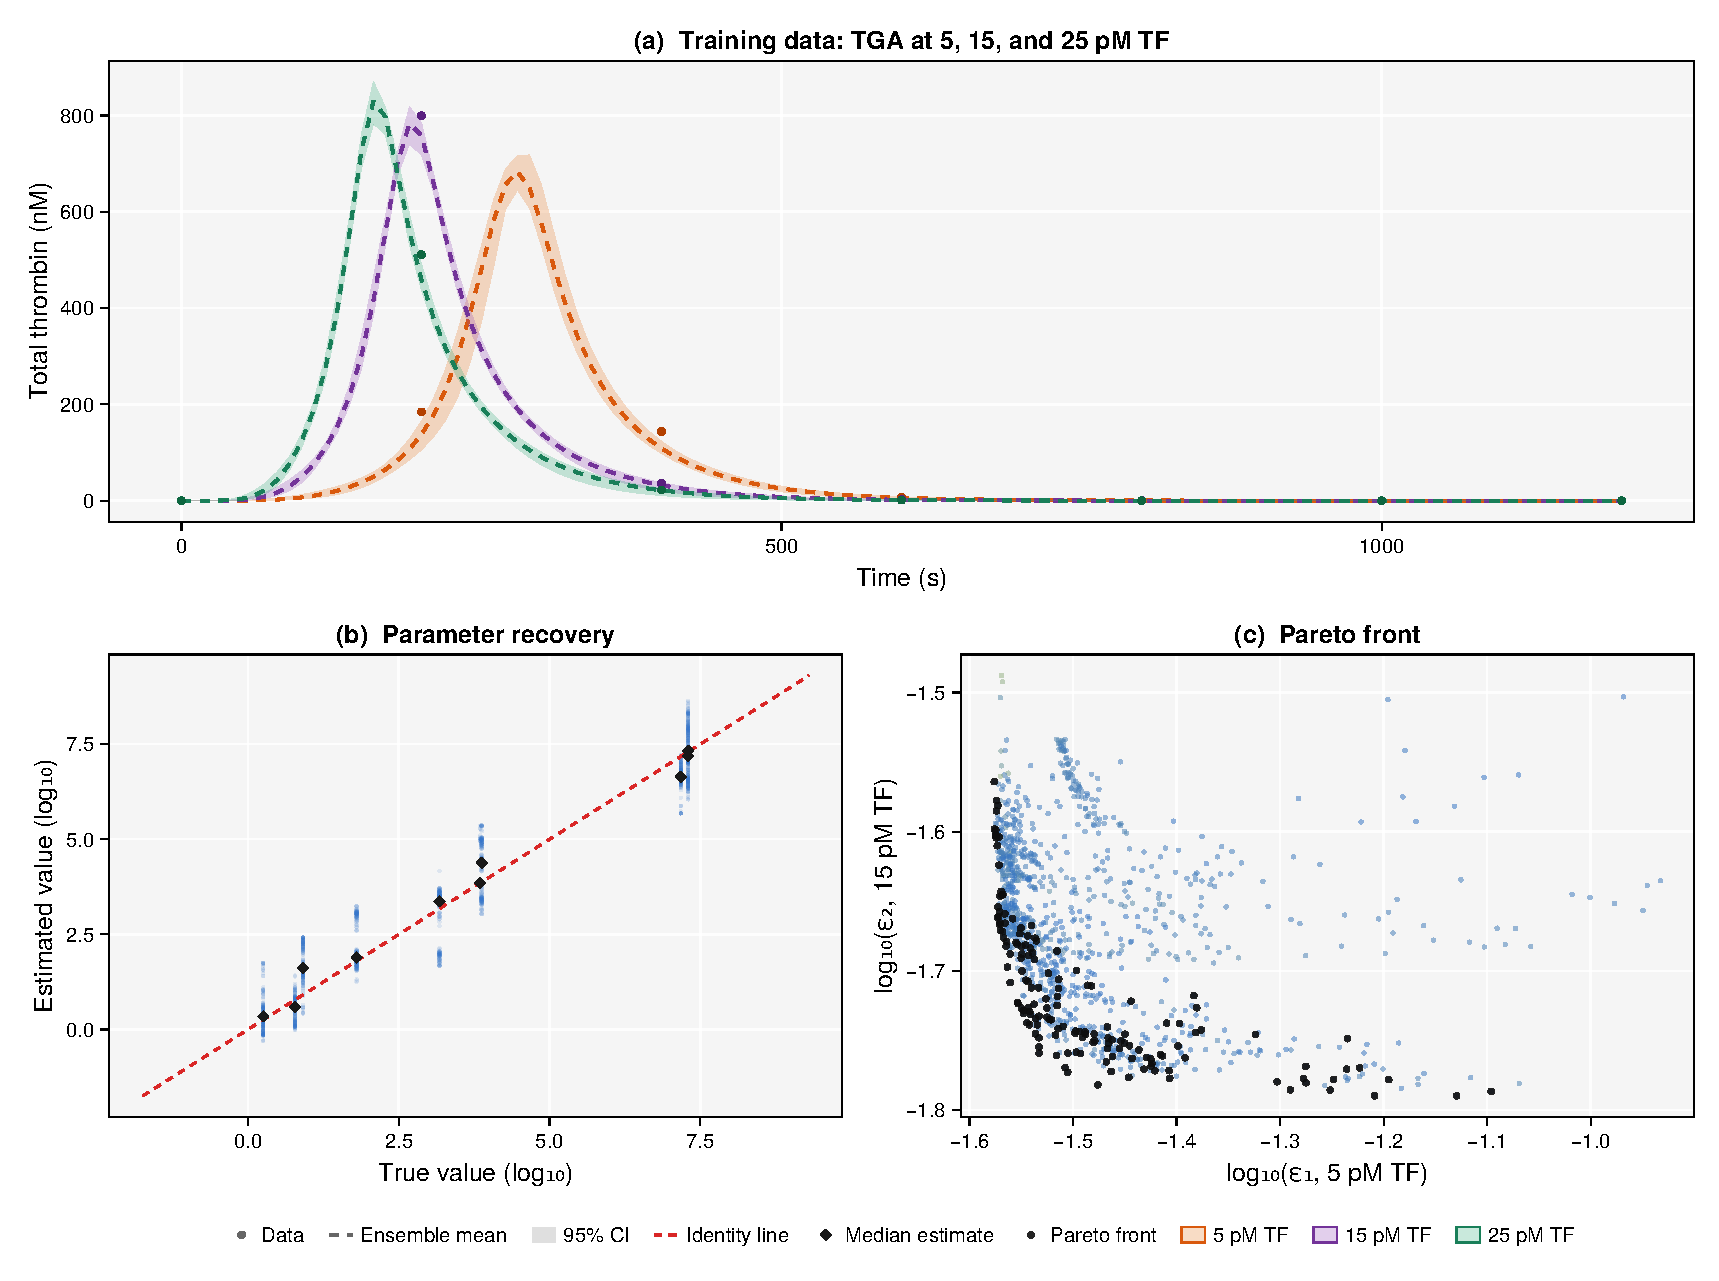
\includegraphics[width=\textwidth]{figures/fig_coagulation.pdf}
\caption{Ensemble estimation for the Hockin--Mann blood coagulation model (34 species, 10 estimated rate constants, 3 objectives).
(a,b)~Total thrombin concentration versus time at 5~pM and 25~pM tissue factor; the blue dashed line is the ensemble mean, the shaded region is the 95\% CI, and black points are noisy data.
(c)~Parameter recovery: estimated versus true rate constants in log-space; the dashed red line is the identity and diamonds show the median ensemble estimate.
(d)~Pareto front projection ($\varepsilon_1$ vs.\ $\varepsilon_2$), with rank-zero solutions in black.}\label{fig:coag}
\end{figure}

\begin{figure}[p]
\centering
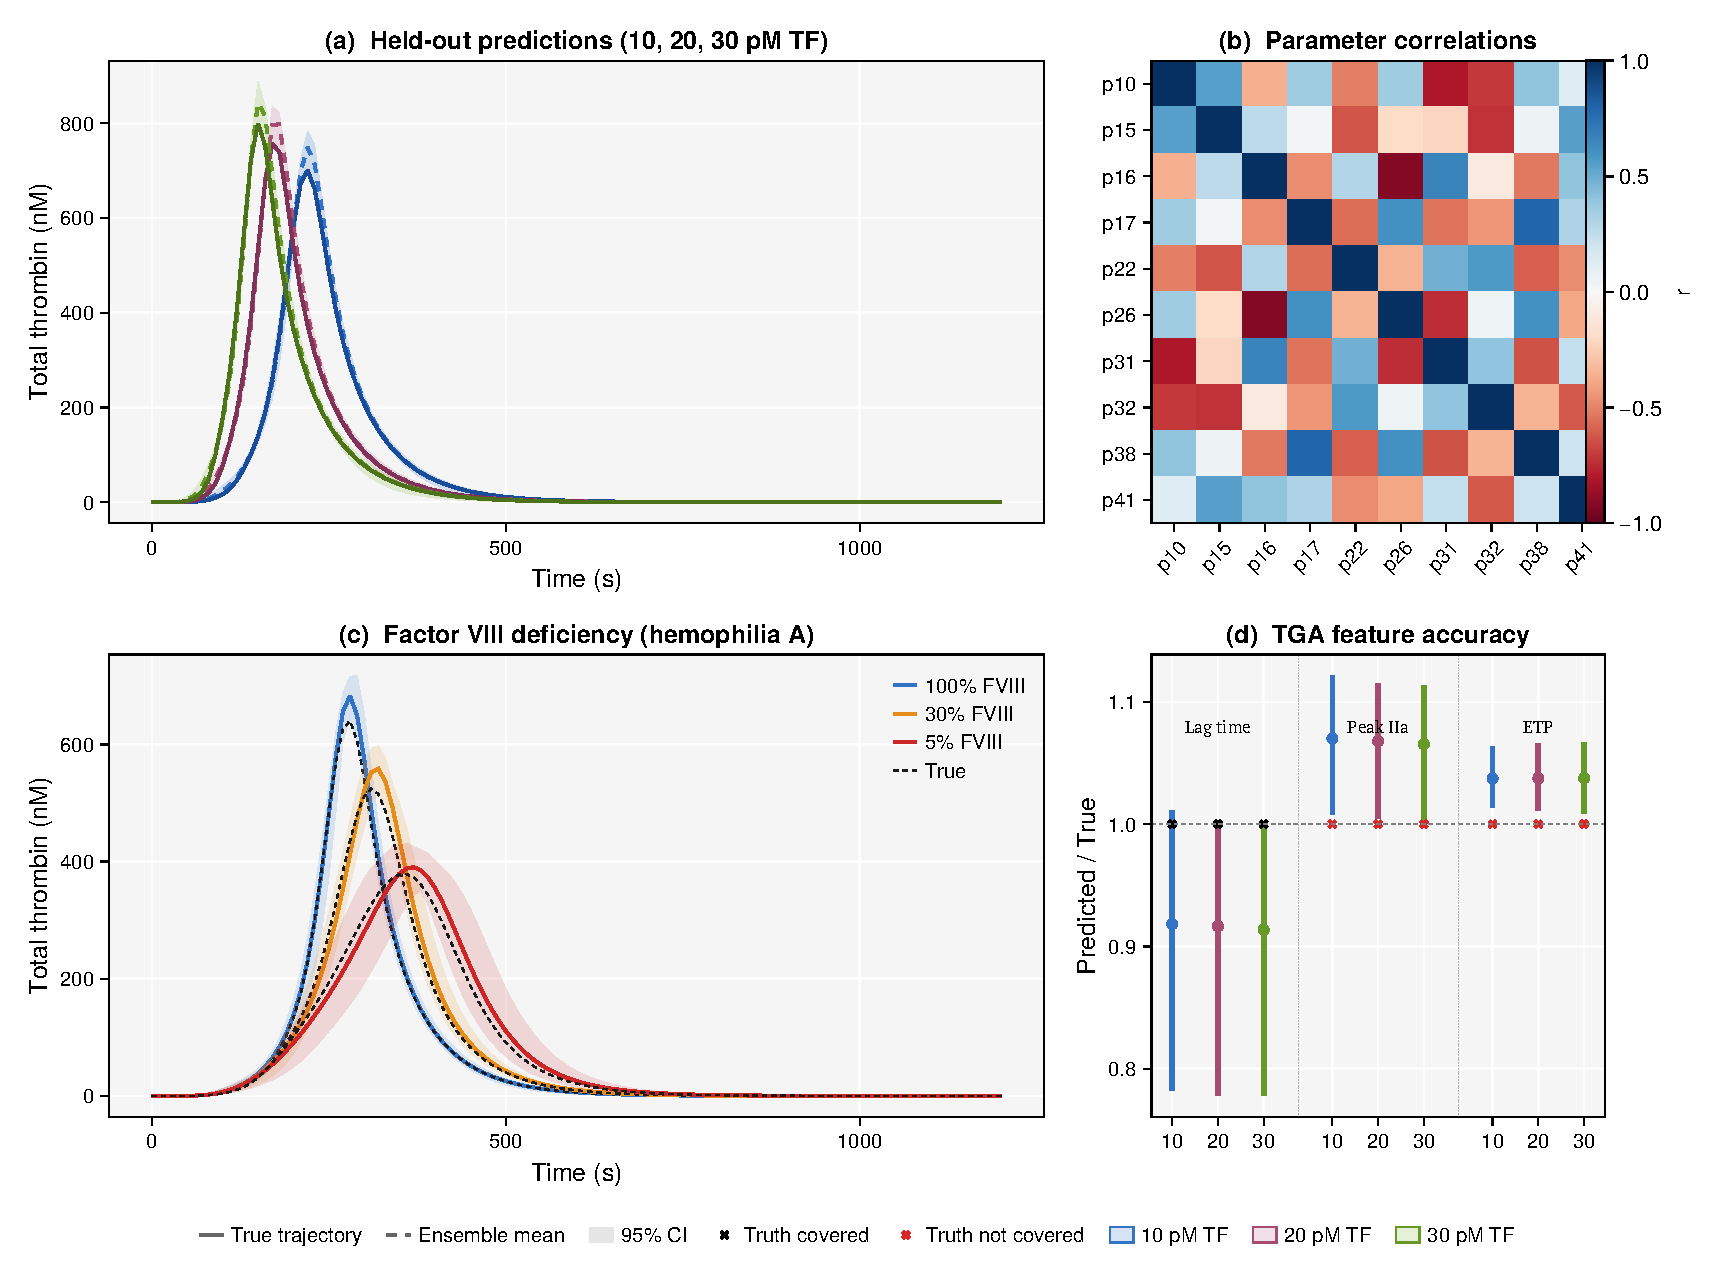
\includegraphics[width=\textwidth]{figures/fig_ensemble_insights.pdf}
\caption{Downstream ensemble analysis for the coagulation model.
(a)~Held-out prediction at 1~pM TF (not used during training): the ensemble mean (blue dashed) and 95\% CI (shaded) bracket the true trajectory (black), while the single best-fit (red dotted) provides no uncertainty information.
(b)~Pairwise parameter correlation heatmap revealing compensatory relationships; strong negative correlations (e.g., extrinsic Xase $k_{\text{cat}}$ vs.\ prothrombinase $k_{\text{cat}}$, $r = -0.80$) indicate parameters that trade off against each other.
(c)~Patient-specific predictions for Factor~VIII deficiency (hemophilia~A) at 100\%, 30\%, and 5\% of nominal FVIII levels; ensemble prediction bands capture the dose-dependent reduction in peak thrombin with calibrated uncertainty, and true trajectories (black dashed) fall within all three bands.}\label{fig:insights}
\end{figure}

\begin{figure}[p]
\centering

\includegraphics[width=\textwidth]{figures/fig_comparison.pdf}
\caption{Comparison of ParetoEnsembles.jl (left) and NSGA-II (right) on (a,b)~Binh--Korn and (c,d)~Fonseca--Fleming at matched evaluation budgets ($\sim$110{,}000).
ParetoEnsembles.jl retains a cloud of near-optimal solutions (blue) in addition to the Pareto front (black), while NSGA-II returns only the non-dominated front.
The dashed red curve in (c,d) is the theoretical Fonseca--Fleming front.}\label{fig:comparison}
\end{figure}

\begin{figure}[p]
\centering
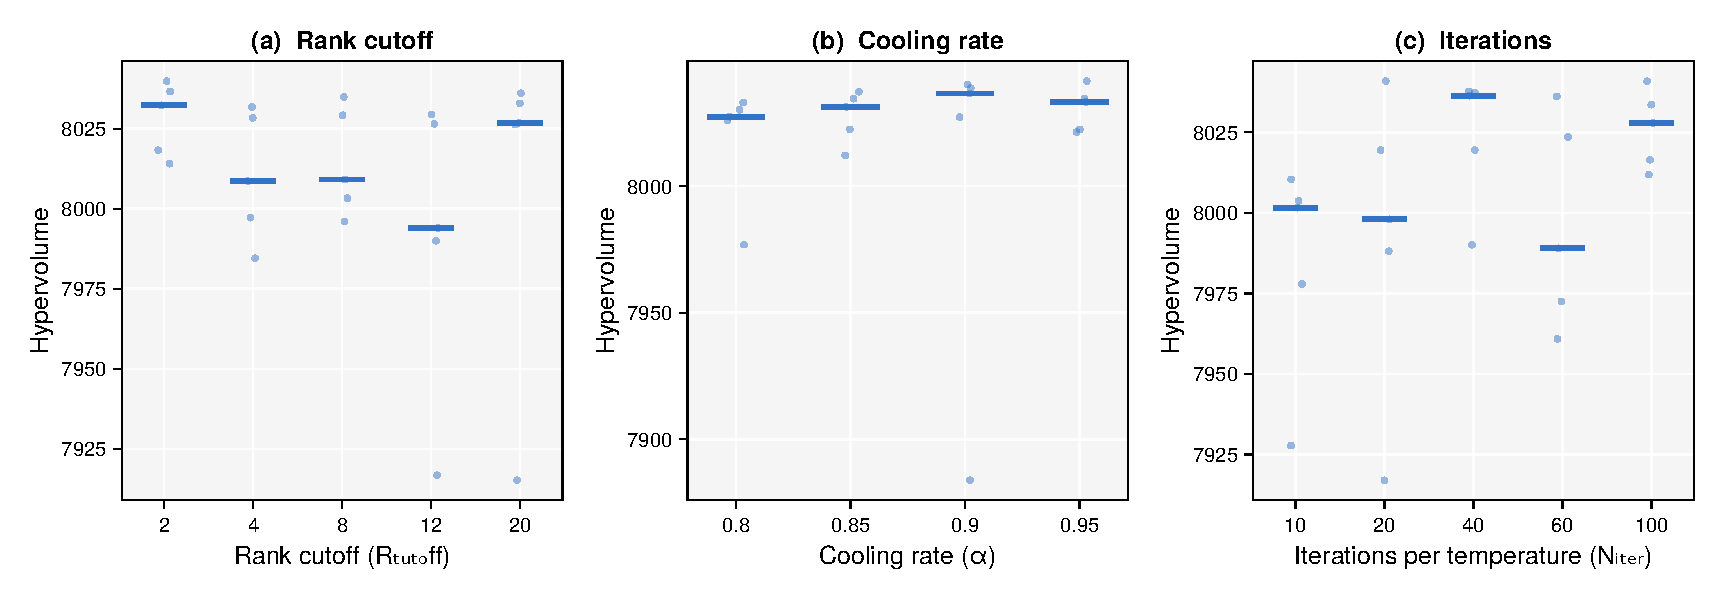
\includegraphics[width=\textwidth]{figures/fig_sensitivity.pdf}
\caption{Hyperparameter sensitivity on the Binh--Korn benchmark.
Median hypervolume (line) with interquartile range (shaded band) over 5 replicates.
(a)~Rank cutoff $R_{\text{cutoff}}$, (b)~cooling rate $\alpha$, (c)~iterations per temperature $N_{\text{iter}}$.
Default values for the other two parameters are held constant in each sweep.}\label{fig:sensitivity}
\end{figure}

% ============================================================
% SUPPLEMENTARY MATERIAL
% ============================================================
\clearpage
\appendix
\section*{Supplementary Material}\label{sec:supplementary}

\begin{lstlisting}[caption={Binh--Korn benchmark with ParetoEnsembles.jl.},label={lst:binhkorn}]
using ParetoEnsembles

function objective_function(x)
    f = zeros(2, 1)
    f[1] = 4.0 * x[1]^2 + 4.0 * x[2]^2
    f[2] = (x[1] - 5)^2 + (x[2] - 5)^2
    # penalty for constraint violations
    lambda = 100.0
    v1 = 25 - (x[1] - 5)^2 - x[2]^2
    v2 = (x[1] - 8)^2 + (x[2] - 3)^2 - 7.7
    f[1] += lambda * (min(0, v1))^2
    f[2] += lambda * (min(0, v2))^2
    return f
end

neighbor_function(x) = clamp.(
    x .* (1 .+ 0.05 * randn(length(x))),
    [0.0, 0.0], [5.0, 3.0])

acceptance_probability_function(R, T) =
    exp(-R[end] / T)

cooling_function(T) = 0.9 * T

(EC, PC, RA) = estimate_ensemble(
    objective_function, neighbor_function,
    acceptance_probability_function, cooling_function,
    [2.5, 1.5]; rank_cutoff=4.0,
    maximum_number_of_iterations=40, show_trace=false)

pareto_idx = findall(RA .== 0)
\end{lstlisting}

\begin{lstlisting}[caption={Multi-chain parallel execution on the Binh--Korn problem (requires \texttt{julia -t4}).},label={lst:parallel}]
using ParetoEnsembles

# ... (same callbacks as Listing 1) ...

initial_states = [
    [2.5, 1.5], [0.5, 2.5],
    [4.0, 0.5], [1.0, 1.0]
]

(EC, PC, RA) = estimate_ensemble_parallel(
    objective_function, neighbor_function,
    acceptance_probability_function, cooling_function,
    initial_states;
    rank_cutoff=4.0, maximum_number_of_iterations=40,
    show_trace=false, rng_seed=42)

println("Solutions: ", size(EC, 2))
println("Pareto-optimal: ", count(RA .== 0))
\end{lstlisting}

\end{document}
